\documentclass[12pt, twoside]{article}
\usepackage[letterpaper, margin=1in, headsep=0.5in]{geometry}
\usepackage[english]{babel}
\usepackage[utf8]{inputenc}
\usepackage{amsmath}
\usepackage{amsfonts}
\usepackage{amssymb}
\usepackage{tikz}
\usetikzlibrary{quotes, angles}
\usepackage{graphicx}
\usepackage{enumitem}
\usepackage{multicol}

\newif\ifmeta
\metatrue %print standards and topics tags

\title{Regents Geometry}
\author{Chris Huson}
\date{September 2020}

\usepackage{fancyhdr}
\pagestyle{fancy}
\fancyhf{}
\renewcommand{\headrulewidth}{0pt} % disable the underline of the header
\raggedbottom


\fancyhead[LE]{\thepage}
\fancyhead[RO]{\thepage \\ Name: \hspace{4cm} \,\\}
\fancyhead[L]{BECA / Dr. Huson / Geometry 06-Analytic-geometry\\* pset ID: 88}

\begin{document}

\subsubsection*{6-7EN-Midpoint-graphs}
\begin{enumerate}
\item Given $\overleftrightarrow{AB}$ as shown on the number line, with $A=2$ and $B=8$. Mark and label the midpoint $M$ between $A$ and $B$?\\[20pt] % Midpoint
  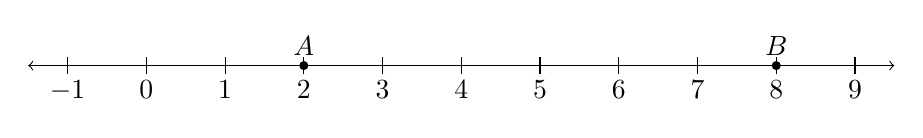
\begin{tikzpicture}
    \draw [<->] (-1.5,0)--(9.5,0);
    \foreach \x in {-1,...,9} %2 leading for diff!=1
      \draw[shift={(\x,0)},color=black] (0pt,-3pt) -- (0pt,3pt) node[below=5pt]  {$\x$};
      \draw [fill] (2,0) circle [radius=0.05] node[above] {$A$};
      \draw [fill] (8,0) circle [radius=0.05] node[above] {$B$};
  \end{tikzpicture}
  
\item On the graph below, draw $\overline{AB}$, with $A(-1,4)$ and $B(5,-2)$, labeling the end points. Determine and state the coordinates of the midpoint $M$ of $\overline{AB}$ and mark and label it on the graph.
  \begin{flushright}
    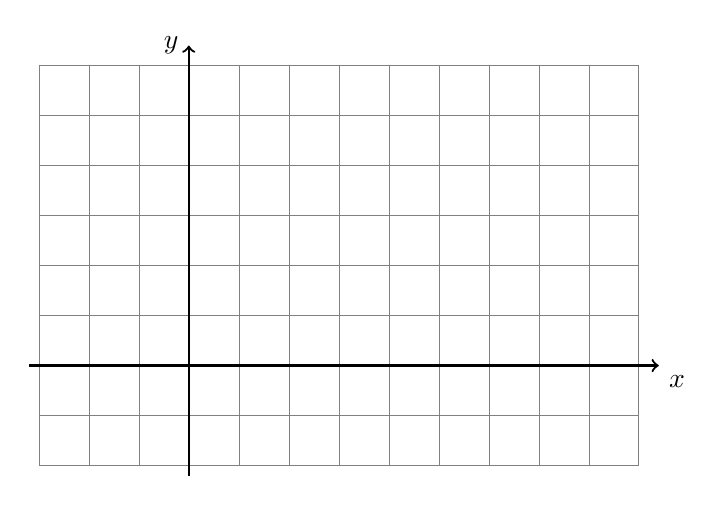
\begin{tikzpicture}[scale=.635]
      \draw [help lines] (-3,-2) grid (9,6);
      \draw [thick, ->] (-3.2,0) -- (9.4,0) node [below right] {$x$};
      \draw [thick, ->] (0,-2.2)--(0,6.4) node [left] {$y$};
    \end{tikzpicture}
  \end{flushright}
  
  
\item On the graph below, draw $\overline{AB}$, with $A(1,2)$ and $B(7,4)$, labeling the end points. Determine and state the coordinates of the midpoint $M$ of $\overline{AB}$ and mark and label it on the graph.
  \begin{flushright}
    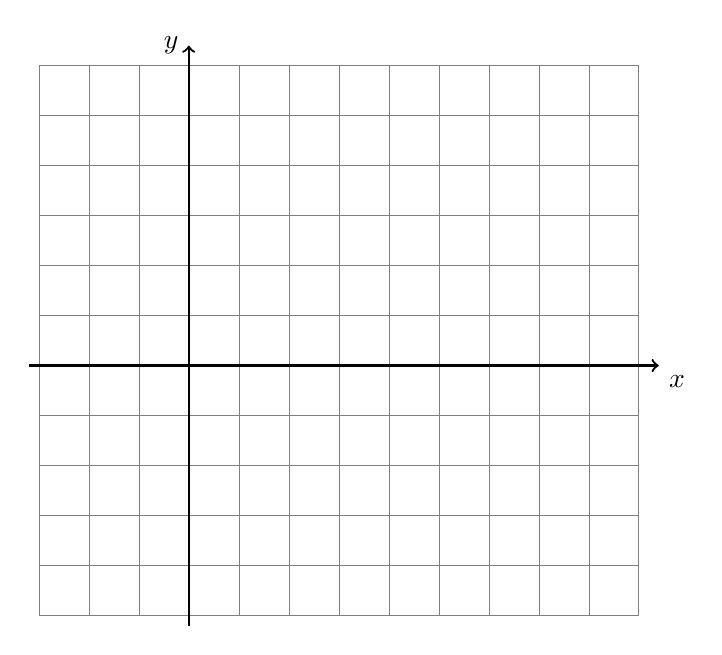
\begin{tikzpicture}[scale=.635]
      \draw [help lines] (-3,-5) grid (9,6);
      \draw [thick, ->] (-3.2,0) -- (9.4,0) node [below right] {$x$};
      \draw [thick, ->] (0,-5.2)--(0,6.4) node [left] {$y$};
    \end{tikzpicture}
  \end{flushright}
  \vspace{1cm}

\newpage
\subsubsection*{Early finishers}
\item Graph and label the two equations. Mark their intersection as an ordered pair.
\begin{multicols}{2}
  $y = x+7$ \\
  $4x+5y=-10$
\end{multicols}     \vspace{2cm}
Are the lines parallel, perpendicular, or neither? Justify your answer.
\vspace{2cm}

\begin{center} %4 quadrant regents grid w T-Chart
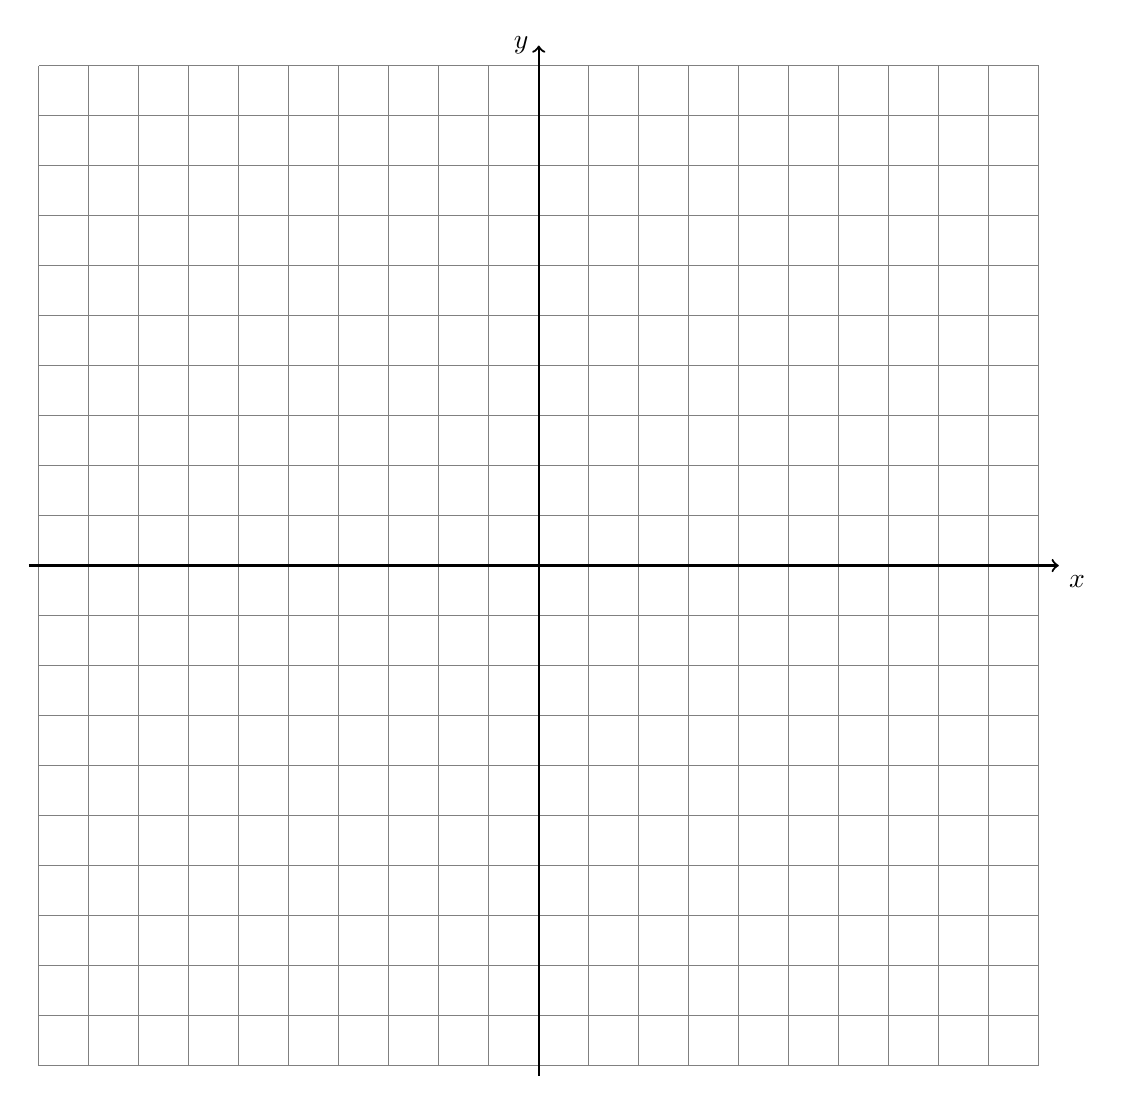
\begin{tikzpicture}[scale=.635]
  \draw [help lines] (-10,-10) grid (10,10);
  \draw [thick, ->] (-10.2,0) -- (10.4,0) node [below right] {$x$};
  \draw [thick, ->] (0,-10.2)--(0,10.4) node [left] {$y$};
\end{tikzpicture}
\end{center}

\end{enumerate}
\end{document}